  %%%%%%%%%%%%%%%%%%%%%%%%%%%%%%%%%%%%%%%%%%%%%%%%%%%%%%%%%%%%%%%%
%                                                              %
%   ECCE Note template
%   v0 produced August 1, 2021
%             
%                                                              %
%%%%%%%%%%%%%%%%%%%%%%%%%%%%%%%%%%%%%%%%%%%%%%%%%%%%%%%%%%%%%%%%

%%  ECCE proposal team: Peter Steinberg (peter.steinberg@bnl.gov)

% C. Fanelli --- Oct 8, re-adapted template
 
                           
\documentclass[12pt,twoside]{article}
%\date{December 1, 2021}

%-----------
\usepackage{array}
\newcolumntype{P}[1]{>{\centering\arraybackslash}p{#1}}
\newcolumntype{M}[1]{>{\centering\arraybackslash}m{#1}}

%%%%%%%%%%%%%%%%
% Adding the include only list allows you to typeset only your
% chapter while maintaining overall page numbers and references.
% It also shields you from errors in other chapters as you go along.
% You need to typeset the whole thing once though. 

%\includeonly{title_page,daq_trig/daq_trig}

%%%%%%%%%%%%%%%%%%  header  (packages, 

\usepackage{amssymb}
%% \usepackage{amsthm}

\usepackage{caption}
\usepackage{xspace}
\usepackage{longtable}
\usepackage{pdflscape}
\usepackage{multirow}
\usepackage{ragged2e}
\usepackage{booktabs}
\usepackage{hyperref}
\usepackage{tikz}
\usetikzlibrary{arrows,chains,shapes,matrix,scopes,positioning,fadings,backgrounds,fit,mindmap,trees,decorations.markings,decorations.pathreplacing,calc}
\usetikzlibrary{decorations.pathmorphing,decorations.markings,trees,arrows.meta}

\newcommand{\eA}{\mbox{$e-{\rm A}$}}
\newcommand{\jpsi}{\mbox{$J/\psi$}}
\newcommand{\mrwell}{\mbox{$\mu$RWELL}\xspace}
\newcommand{\PbWOiv}{\mbox{PbWO$_4$}\xspace}
\newcommand{\geant}{\mbox{\sc Geant4}\xspace}

%% The lineno packages adds line numbers. Start line numbering with
%% \begin{linenumbers}, end it with \end{linenumbers}. Or switch it on
%% for the whole article with \linenumbers.
\usepackage{lineno}


\title{ECCE Computing Plan}
\author[1,2,3]{Jan C. Bernauer}
\author[4]{Cameron Dean}
\author[5]{Cristiano Fanelli}
\author[6]{Jin Huang}
\author[6]{Kolja Kauder}
\author[7]{David Lawrence}
\author[6,8]{Joseph D. Osborn}
\author[5]{Christoph Paus}


\affil[1]{Department of Physics and Astronomy, Stony Brook University, Stony Brook, NY 11794}
\affil[2]{RIKEN BNL Research Center, Upton, NY 11973}
\affil[3]{Center for Frontiers in Nuclear Science, Stony Brook University, Stony Brook, NY 11794}

\affil[4]{Los Alamos National Laboratory, Los Alamos, NM 87545}
\affil[5]{Laboratory for Nuclear Science, Massachusetts Institute of Technology, Cambridge, MA 02139}
\affil[6]{Brookhaven National Laboratory, Upton, NY 11973}
\affil[7]{Thomas Jefferson National Accelerator Facility, Newport News, VA 23606}
\affil[8]{Oak Ridge National Laboratory, Oak Ridge, TN 37830}




\begin{document}
%\frontmatter
%\pagestyle{empty} %Setting this to empty removes page numbers
\pagestyle{empty}
%%%%%%%%%%%%%%%%%%%%%%%%%%%%%%%%% title page
\renewcommand*\familydefault{\sfdefault}
{\sffamily
\vfill
\vspace{4cm}
\begin{figure}[H]
  \begin{center}
  \includegraphics[width=0.3\linewidth]{figs/ecce-logo.png}
\end{center}
\end{figure}

\begin{center}
  \large
  {\LARGE{ECCE Computing Plan}}

  \begin{tabular}{cc}
& Preliminary
%A full-acceptance detector at the EIC based on the BaBAR magnet 
\\
&October 23, 2021 \\
  \end{tabular}
  \end{center}

\vspace{15cm}
\hspace*{0pt}\hfill ecce-note-comp-2021-01 \\
\hspace*{0pt}\hfill v0.0
\vspace{-15cm}

\vspace{1cm}

\begin{figure}[H]
  \begin{center}
    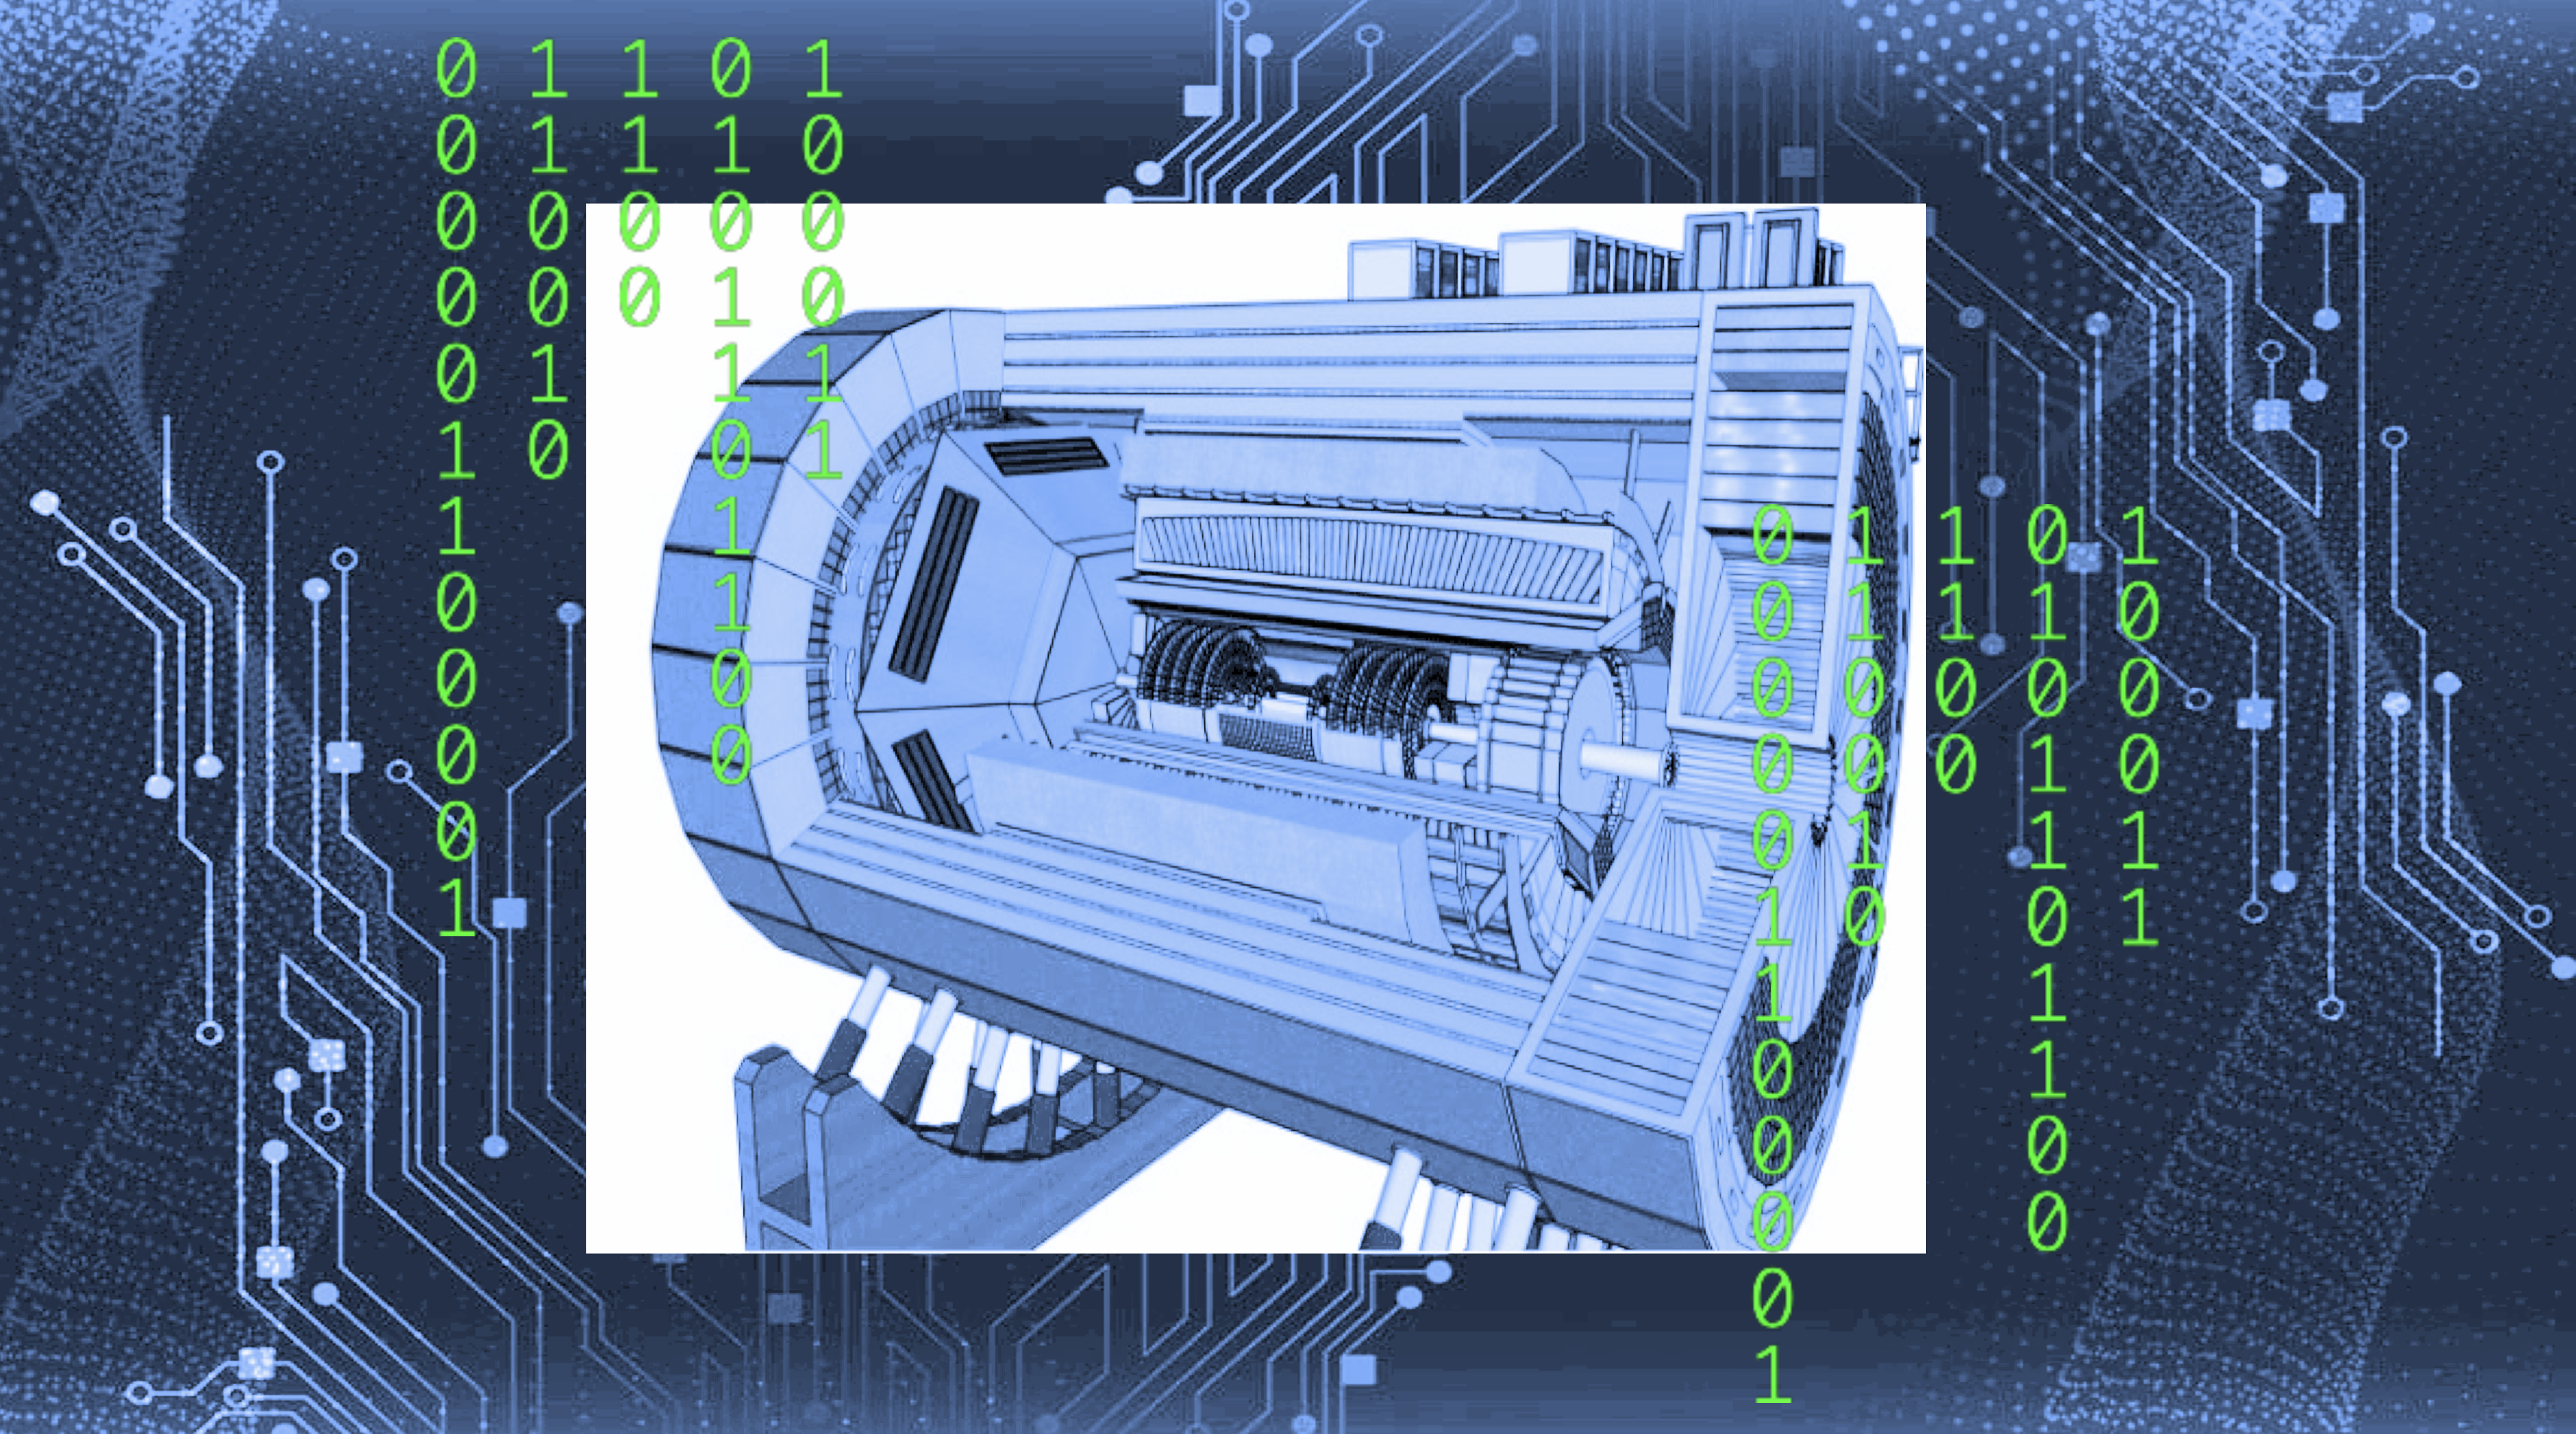
\includegraphics[width=0.7\linewidth]{figs/ECCE_computing_fig.png}
  \end{center}
\end{figure}
}


\vfill
\renewcommand*\familydefault{\rmdefault}


\cleardoublepage
\pagestyle{plain}
\maketitle
\pagenumbering{roman}

%\setcounter{page}{1}

%\clearpage
%\cleardoublepage

%\resetlinenumber


%\cleardoublepage

%\mainmatter

%\renewcommand{\thepage}{\arabic{page}}
%\setcounter{chapter}{0}
%\setcounter{page}{1}

%%%%%%%%%%%%%%%%%%%%%%%%%%%%%%%%% 
\begin{abstract}
%\section* {Executive Summary}
\label{sec:ExecutiveSummary}

% Executive Summary

The ECCE consortium plans to deploy a federated computing model for the EIC where multiple facilities are used. ECCE recognizes the need for a global EIC model and intends to fully participate in the design and implementation of such a system. A similar strategy has been successfully deployed by the LHC in the form of the Worldwide LHC Computing Grid (WLCG)~\cite{SHIERS2007219}. ECCE has developed a tiered ``Butterfly'' model for EIC computing that was inspired by the WLCG model, but updated to better reflect the computing landscape anticipated for the EIC. In this model, the EIC detector supplies the data, but the SDCC at BNL is treated as one of a pool of sites used for long term storage and compute. Both SDCC and JLab would be considered as \emph{Echelon 1} sites with the ability to add others as appropriate. Raw data would be distributed amongst multiple \emph{Echelon 2} sites for processing with the processed data being returned to Echelon 1. Researchers would directly access the processed data at the Echelon 1 sites.

We have adopted a fixed-latency offline computing model where both the final calibration and reconstruction of raw data occur within 2-3 weeks of acquisition. During this period, raw data will be buffered on disk at all of the Echelon 1 sites, along with permanent archival copies on tapes. Final calibration will be performed semi-automatically including accumulating sufficient data for tracker alignment and energy scale calibration of the calorimeters. AI/ML will be integrated throughout this model. After calibration, data processing  will be released to multiple sites including HTC facilities at both Echelon 1 and 2 sites. We expect that the produced simulation sample will focus on 10\% of the EIC collision cross-section that is directly relevant for the signal and background of the core ECCE physics program. These physics processes will be simulated to $O(10)$~times the statistics in real data to constrain systematic uncertainty from the simulated sample to be much smaller than the data statistical uncertainty.

A summary of the anticipated resource requirements can be seen here in table \ref{tab:computing-integrated_luminosity_by_year}.


\begin{table}[htb!]
    %\centering
    \hskip-0.8cm
    \begin{tabular}{c|c|c|c}
        \hline
        % \hline
         \textbf{ECCE Runs}       & year-1                & year-2                  & year-3                \\
        \hline
         Luminosity              & $10^{33}\mathrm{cm}^{-2}\mathrm{s}^{-1}$ & $2\times 10^{33}\mathrm{cm}^{-2}\mathrm{s}^{-1}$ & $10^{34}\mathrm{cm}^{-2}\mathrm{s}^{-1}$ \\
        %  \hline
         Weeks of Running        & 10                    & 20                      & 30                    \\
        %  \hline
         Operational efficiency    & 40\%                  & 50\%                    & 60\%                  \\
        %  \hline
        Disk (temporary)  &  1.2PB & 3.0PB & 18.1PB \\
        %\hline
        Disk (permanent)    & 0.4PB & 2.4PB &	20.6PB \\
        %\hline
        %\textbf{TOTAL}          & 1.6PB &	5.4PB &	38.7PB \\
         Data Rate to Storage    & 6.7Gbps               & 16.7Gbps                & 100Gbps               \\
        %  \hline
         Raw Data Storage (no duplicates) & 4PB          & 20PB                    & 181PB                 \\
        %  \hline
        %  Total Storage (no duplicates) & 4.4PB           & 22PB                   & 200PB                  \\
        %  \hline
        \hline
        Recon process time/core	& 5.4s/ev	& 5.4s/ev	& 5.4s/ev \\
        % \hline
        Streaming-unpacked event size	& 33kB	& 33kB & 33kB \\
        % \hline
        Number of events produced &	121 billion	& 605 billion & 5,443 billion \\
        % \hline
         Recon Storage          & 0.4PB                  & 2PB                    & 18PB                   \\
        %  \hline
        % CPU-core hours (recon-only, 1 pass)	& 24Mcore-hrs	& 121Mcore-hrs &	1089Mcore-hrs \\
        % \hline
        % CPU-core hours (calib-only) &	1.2Mcore-hrs &	6.0Mcore-hrs &	54.4Mcore-hrs \\	
        % \hline
        CPU-core hours (recon+calib)	& 191Mcore-hrs	& 953Mcore-hrs &	8,573Mcore-hrs \\
        % \hline
        2020-cores needed to process in 30 weeks	& 38k &	189k &	1,701k \\
        % \hline
        \hline
   \end{tabular}
    \caption{Estimate of raw data storage and compute needs for first 3 years of ECCE,  assuming ramp up to full luminosity by year 3. 
    % Numbers for the first two years are estimated for the purposes of this exercise and do not come from an external source. n.b. each value represents \emph{only} the needs for data produced in that year and \emph{not} a cumulative total.
    }
    \label{tab:computing-integrated_luminosity_by_year}
\end{table}

\end{abstract}
\clearpage
\setcounter{tocdepth}{3}
\tableofcontents
\clearpage
\pagenumbering{arabic}
\setcounter{page}{1}

\section {Introduction}
\label{sec:introduction}

%\textbf{\emph{David L.}}

This document presents a proposed computing plan for the ECCE detector at the EIC\cite{eic_yellow_report_v1_1}. This includes estimates of the rates from the detector, the pipeline for processing and storing the data, and how the collaboration members will access the data. Software systems for monitoring, calibration, reconstruction, and analysis are discussed. Estimates of the computing and storage requirements are included.

At this point in time ECCE is still in the proposal stage. The development is being done by the ECCE proto-collaboration. Many details regarding the data pipeline and software systems have not been fully fleshed out. It is anticipated that once a formal ECCE collaboration is established that more rigorous designs will be developed. 

The EIC is anticipated to start producing data approximately a decade from now. As such, it will introduce new paradigms in large scale Nuclear Physics experiments. While we attempt to include some forward thinking plans in this regard, we necessarily do need to rely on past experience with other large experiments such as sPHENIX\cite{sphenix_computing_plan_2019} and LHCb\cite{CAMPORAPEREZ2016280} to serve as guides.

% temporarily commented --- CF
%\section {Artificial Intelligence / Machine Learning} %/Machine Learning
%\label{sec:ai}
%\textbf{\emph{Cristiano/Will}}

%\emph{This is intended to be a fairly brief section.
%AI/ML is expected to be integrated into all aspects of the Computing Plan so should appear throughout the document.
% }


%EIC 
%%has the possibility to incorporate AI from the start and 
%could be one of the first large-scale experiments where AI is systematically employed from the detector and design 

The EIC can be one of the first large-scale experiments to systematically incorporate and employ Artificial Intelligence (AI) in its program, starting from the detector design and R\&D phases. 
The relevance of AI for the EIC has been highlighted among the \textit{Opportunities for Computing} of the EIC Yellow Report \cite{eic_yellow_report_v1_1}.

ECCE recognizes the important role that AI can play at various stages of the future EIC experiment and includes in its structure a working group dedicated to AI-based applications. 
As a result AI permeates all aspects of this Computing Plan and appears throughout the whole document.

The first workshop on Artificial Intelligence for the Electron Ion Collider (AI4EIC) held at CFNS in September 2021 \cite{AI4EIC_workshop} has been a fundamental venue for the EIC community to start addressing how AI might contribute to advance research, design and operation of the future EIC across all the phases of the EIC schedule (see \cite{AI4EIC_future}).
%---- structure of AI4EIC 
The workshop was structured into different sessions focusing on experimental applications of AI for \textit{Accelerator and Detector Design}, \textit{Simulations}, \textit{Reconstruction and Analysis}, \textit{Accelerator and Detector Control}, \textit{Detector Readout} and \textit{Computing Frontiers}. 
%
As a result of this discussion it turned out AI techniques are expected to play a role since the design and R\&D phases of EIC. 
It is in fact clear the advantage of AI techniques in searching the optimal solutions in a complex multi-dimensional parameter space such as in the design of a detector. Detector design requires accurate simulations based on Geant4 \cite{ALLISON2016186}. Those simulations are typically compute intensive and another advantage of using AI is minimizing the computing budget needed to come up with an optimal solution (see, \textit{e.g.}, the results of an AI-supported design of a complex detector system like the dual-RICH \cite{cisbani2020ai}).
%AI can be also utilized for the optimization of materials used within detectors for improved performance. 

%Simulations - fast simulations - ATLAS example 

%Reconstruction - EIC detector has unique features. The backbone of PID is Cherenkov detectors. Compute intensive simulations and complex pattern recognition problems for imaging Cherenkov detectors like DIRC.  

%AI is also expected to play a role in high-level physics analysis, for example in jet physics (cite ML4JETS) to empower taggers for boosted jets and identify quark flavor within the jets.  

% EIC can be one of the first ``automated''/autonomous experiments (see Control Session) control workflows 

% Streaming readout at EIC will further the convergence of online and offline analysis: AI will play a major role in providing fast alignment/calibration/reconstruction for near real-time analyses.

% What opportunities from “computing frontiers” in > 2030? 


--- references to next sections go here ---

--- few sentences to uncomment --- 

--- Will: any addition?

%---- some numbers from:
%%CPU Resources
%%ECCE Tracker Optimization (Cristiano/Karthik)
%%DIRC Optimization Framework # of compute hours/configuration (Will/Andru)
%%Dual Rich (what used for the study in paper) (Cristiano)
%%General purpose simulation for generating training samples for projects listed below
%%???
%%GPU Resources
%%CLAS12 Tracking  (Gagik/ODU Students)
%%Hydra Online Monitoring Training (Kishan/Thomas)
%%Online track reconstruction?
%%???

%---- final summaries, keywords and citations 




% temporarily commented --- CF
%\section {Detector and Program Development}
%\label{sec:detector_development}
%\subsection{Detector Optimization}
\label{sec:codesign}
\textbf{\emph{Cristiano}}


%The optimization is an essential part of the R\&D and design process.
%An unprecedented study in detector design using AI has been accomplished and a framework for multi-objective optimization of the ECCE design has been developed. 
%Our approach deals with a complex optimization in a multidimensional design space driven by multiple objectives that encode the detector performance, while satisfying several mechanical constraints. 
%%This approach can be further utilized 
%%We describe our strategy and show preliminary results for the Si tracking system. 


% Future: scaling workflow on HPC system 

\section {Online}
\label{sec:online}
%- - - - - - - - - - - - - - - - - - - - - - - - - - - - - - - - - 
\subsection{Data Acquisition}

\textbf{\emph{Jan B.}}

\emph{This section does not need to go into complete detail on the DAQ system (that should be in a different document). This should include the global picture (see slide 5 of Jin's intro talk at AI4EIC or slide 3 of Fernando's talk). What is needed here is the expected overall data rate and how many streams. The current plan is to implement a first stage HLT which may or may not require full event building. This section will need to include an estimate of how much reduction the first stage HLT will provide (i.e. what is the data rate going into the calibration system.}

\emph{Also, do we implement the first stage HLT in FPGAs or on CPU/GPU? Need estimates on how much compute resource will be needed for first stage HLT.}

%--------------------------------------------------------------------
Figure \ref{fig:data_acquisition_diagram} illustrates a concept of the data acquisition system with some estimated rates.

\begin{figure}[hbt!]
 \begin{center}
   \raisebox{0.5mm}{\includegraphics[trim=50 30 50 30, clip, width=0.99\linewidth]{figs/figure_data_acquisition_diagram.pdf}}
  \caption[Data Acquisition Diagram]{\label{fig:data_acquisition_diagram} Diagram of a Data Acquisition system. This is reproduced from slides shown at AI4EIC 2021\cite{EIC_readout_overview_AI4EIC_2021}. }
 \end{center}
\end{figure}

%- - - - - - - - - - - - - - - - - - - - - - - - - - - - - - - - - 
\subsection{Monitoring}

Hydra\cite{Hydra2021}



\section {Offline}
\label{sec:offline}

%\textbf{\emph{David L.}}

Offline software encompasses many aspects of the experiment. This includes a number of systems, each of which requires either new development or implementation of existing systems using dedicated experts(s). These include:

\begin{itemize}
    \item Calibration system and database
    \item Reconstruction framework
    \item Reconstruction algorithms
    \item Simulation
    \item Offline Monitoring system
    \item Reconstruction workflow (HPC/HTC job management)
\end{itemize}

We intend to develop an offline computing model that aims for ``real time analysis'' that performs a single reconstruction pass on the data to produce reduced DSTs that are available for physics analysis on the time scale of a few weeks. In this description, the single reconstruction pass includes any relevant calibrations that are determined from specific calibration data sets. 

In the following sections we describe some of the above systems that will constitute larger efforts in terms of person-hours. It should be noted that at this time certain technology choices seem likely (e.g. GEANT4~\cite{ALLISON2016186}). However, others such as the choice of database systems, file formats, and software frameworks are purposefully left unspecified at this point in time.

%- - - - - - - - - - - - - - - - - - - - - - - - - - - - - - - - - 
\subsection{Reconstruction}\label{subsec:reconstruction}

%\textbf{\emph{Joe O.}}

In the past several decades, many reconstruction frameworks have been developed by different experiments within both HEP and NP. Several features stand out as common to all of these, which the ECCE software framework must utilize. The most important of these are modularity and user friendliness, as any large HEP/NP collaboration will necessarily comprise many hundreds of scientists with varying levels of software expertise. Therefore, these, and other generic features of excellent software, will be essential. It will additionally be imperative to recognize that software technologies change rapidly, and the ability for the software ecosystem to pivot with ease will be essential. As an example, while \texttt{git} is the de facto modern standard for code versioning and storage, it is impossible to say what versioning technologies will exist ten or more years from now when the EIC will be taking data. ECCE has not committed itself to a particular software ecosystem yet; however, these discussions will need to begin in early 2022 as these decisions will need to be made in preparation for development of a TDR.

One of the trademarks of excellent reconstruction software is reproducibility. ECCE will archive several daily builds that will provide users with the latest snapshot of the software; additionally, weekly builds that persist for longer periods of time will allow tracking of code evolution. In conjunction, special tagged production builds will be archived for large centrally produced data samples, such as those that were produced in preparation for the ECCE proposal. Currently the tagged releases are performed based only on time (e.g. weekly builds). Future software versions will consider implementing modern versioning practices such as semantic versioning~\cite{semantic}. In addition to archived builds, continuous integration is another tool ensuring reproducibility. ECCE does not currently deploy robust continuous integration; however, automated tools enabled by services such as Jenkins or GitLab Runners will be deployed utilizing code checking tools and benchmark analyses. 

Making software user friendly requires that it is distributed in a convenient way. Currently the ECCE framework is distributed with \texttt{cvmfs}, a package managing software developed at CERN~\cite{cernvm}, while the software environment is containerized and deployed with Singularity~\cite{singularity}. Any software system that ECCE decides on will necessitate these tools for distribution, to ensure that all users can easily access the software and that a reproducible environment is available when deploying offline analysis and simulation in a federated computing architecture.

The role of hybrid architectures should also be considered in the ECCE reconstruction framework. Specifically, the use of GPU architectures will be important both for integrating machine learning into reconstruction workflows as well as generically taking advantage of the significant computational speed improvements that GPUs can provide. This integration has the added benefit of potentially utilizing the various leadership computing facilities that are available at national laboratories around the country, for more see Section~\ref{sec:offsite}.


Based on the experience of other experiments, reconstruction software should also take advantage of common software projects that are deployed across the world. For example, the A Common Tracking Software (ACTS) package, initially designed for use at the HL-LHC, has been implemented into the sPHENIX track reconstruction framework~\cite{Osborn:2021zlr}. Several collider-physics-based open source projects exist within the broader HEP community and have recently grown in in their user base, examples include ACTS~\cite{Ai:2021ghi}, Rucio~\cite{Barisits:2019fyl}, PanDA~\cite{pandaDocs}, Fun4All~\cite{fun4allGithub}, JANA~\cite{jana2_chep19}, Gaudi~\cite{Gaudi}, and others. These should be evaluated for use within the ECCE software stack in early 2022 as a part of the decision making process for the future of the offline software framework.

%\emph{This section should focus on the features that are needed for the reconstruction framework. This should avoid committing to a particular software package at the moment. That is a discussion/decision we should have in early 2022 and I think this section can state that explicitly. Features that will be needed should be driven by HTC system requirements. Specifically, the ability to parallelize both vertically and horizontally. Use of heterogeneous hardware. Containerization and distribution(e.g. CVMFS) should also be discussed. Another general issue is how to distribute calibration and meta-data to potentially 100k jobs without them all hitting a single central server at once. Provisioning for multiple, replicated servers would be appropriate here.}

%\emph{This will need standard statements about modularity and user friendliness of the framework. I think it would be safe to state that we expect the primary language to be C++ while not excluding the integration of other languages.}

%\emph{Need estimates of total CPU}

%- - - - - - - - - - - - - - - - - - - - - - - - - - - - - - - - - 
\subsection{Calibration}

%\textbf{\emph{Jin H.}}

%\emph{The calibration system will be integrated into the Online/DAQ with the goal being to to produce calibrations in ``real time'' a'la LHCb. This should give some details included expected latency/disk space, etc.}

%\emph{Another important aspect will be how the calibration DB identifies chunks of time. We discussed making boundaries at lumi blocks corresponding to electron beam fills that are expected to happen at about 1Hz.}

%\emph{Need estimate of size of calibration DB/year of operation. This will be small compared to raw data, but since it will be maintained by different machines and software, it is worth breaking out.}

%---------- Pasting Jin's section from the old overleaf (C. Fanelli)


% \textbf{\emph{Jin H.}}

% \emph{The calibration system will be integrated into the Online/DAQ with the goal being to to produce calibrations in ``real time'' a'la LHCb. This should give some details included expected latency/disk space, etc.}

% \emph{Another important aspect will be how the calibration DB identifies chunks of time. We discussed making boundaries at lumi blocks corresponding to electron beam fills that are expected to happen at about 1Hz.}

% \emph{Need estimate of size of calibration DB/year of operation. This will be small compared to raw data, but since it will be maintained by different machines and software, it is worth breaking out.}


Timely delivery of high-quality calibration is one of the main challenges for EIC experiments, in particular given that many EIC measurements will be systematic uncertainty driven \cite{eic_yellow_report_v1_1}. ECCE adopts a fixed-latency production model, which requires the final calibration within 2-3 weeks of data taking. This leads to the design of a semi-automatic calibration workflow with minimal human intervention. 

\subsubsection{Calibration workflow}


Similar to the architecture of the sPHENIX computing model, we envision offline computing center will provide a large incoming data buffer (e.g. 20PB as in the sPHENIX) that allows raw data to be used for reconstruction within 2-3 weeks of data taking, during which calibration will take place. The calibration tasks and time scale are dependent on the detector subsystems: 

\begin{itemize}
\item Tracker hit: amplitude and time offset of each tracker channel will be aligned to a uniform response using an ensemble of collisions. We expect the initial calibration is delivered within two weeks of data taking with frequent checks and updates when needed. 
\item Particle ID, which will require gain and time calibration
\begin{itemize}
  \item The single-photon and multi-photon per pixel hit from signal hit and noises will be used to set the gain. We expect a rapid turnaround for calibration and monitoring of the gain ($<$1 day)
  \item The time offset calibration will be initially set by calibration pulse lasers, which is applied before the physics data taking. The final alignment requires events with a high multiplicity of tracks and aligning their projected collision time by adjusting timing shifts for each sensor, which will be part of the 4D alignment to be discussed at the end of the list. 
\end{itemize}
\item Calorimetric calibration, which will focus on gain calibration
\begin{itemize}
  \item Leading order calorimetric energy scale calibration will be performed during the production stage using the block 
  \item QA database and SiPM gain database. 
  \item The first iteration for the calorimetric energy scale will be based on cosmic data during the construction phase (e.g. sector testing) and pre-collision cosmic runs. This is expected to be completed before physics data taking
  \item The second iteration of tower-by-tower energy scale variation calibration will be matching the energy slope of the calorimeter tower energy spectrum for the same eta slice.   This is expected to be completed within one week of physics data taking
  \item The final energy scale iteration will utilize the collision data: 1) use DIS electron, $\pi^{\circ}$ and $\eta$ to $\gamma \gamma$ decay to set the energy scale for the EMCal, 2) isolated hadronic shower to calibrate the e/h in EMcal and hadronic energy scale in the HCal, 3) single high SIDIS jet production to set calorimetric jet energy scale. This is expected to take one week of data ($O(100)$ Billion events) and one week of calibration. 
  \item During the steady-state running, the tower-by-tower gain drift will be monitored and calibrated using LED flashes and SiPM temperature monitoring, which can be calibrated in about one hour during steady-state running. 
\end{itemize}

\item Full detector alignment: each detector will be surveyed before and after installation which provides the starting point of the alignment. 
\begin{itemize}
  \item The first iteration of alignment will use field-off data and cosmic data to adjust major pieces of the detector component to the final installed location. The time latency needed for this task is limited by the availability of such specialized data, but we expect this step is completed before the physics quality data taken at ECCE
  \item The second iteration requires field-on physics quality collision data to provide the final high precision adjustment for the sensor locations and time offset (for TOF) to a small fraction of the resolution. The first period of magnetic-field-on collision data will be used for this alignment. Generic purpose global alignment package such as Millepede II will be used. It is expected to take two weeks to complete the iteration of alignment and checks. 
  \item Steady-state updates: vertex tracker require O(1)~$\mu$m level of alignment, which could drift over a long period. Therefore, during steady-state running, we expect alignment to be checked every few days and possibly updated every week, depending on the final mechanical stability. We expect steady-state alignment updates can be achieved fast, within one hour (e.g. LHCb vertex tracker is aligned in a few minutes). 
\end{itemize}

\end{itemize}

\subsubsection{Calibration database}

For the ECCE streaming DAQ, we expect the calibration record is time-stamped with a 64-bit beam crossing counter with the start and end time of the validity window. The validity window length will be detector and calibration type-dependent, but we expect they align with the luminosity block of ECCE streaming data that is at the order of magnitude of 1s, at each of the electron ring bunch refills. 

The size of the calibration data is much smaller than the raw data but still sizable. For the highest channel count for the silicon vertex tracker (O(1)B channels), we do not expect it to have frequent calibration as it presents boolean (hit/no-hit) pixel data. In a conservative estimation, consider 300 thousand of the calorimeter, tracker, and PID channels require a frequent (1 per minute) update of a relative gain and time shift, each represented by a 4-Byte float number. This gives an overall calibration dataset size of $O(1)$~TB per run year (8B*(300e3 chan)*60(second)*24(hour)*7(week)*20(PAC run week)). 

The calibration data will be indexed in a relational database. The actual calibration data file can be in a distributed file server (e.g.\ S3 or XROOTD) or in a separated database table, depending on the size per entry and frequency of calibration update. The separation of index database and calibration data payload allows for efficient database implementation management that is capable of accommodating a possible large size of the calibration data. This approach is being deployed in the sPHENIX fixed latency calibration and reconstruction.

At the start of a production job, the job manager will pull the calibration data relevant for the job into the local disk buffer according to the index table. Then the database is disconnected and job processing starts to efficiently utilize the connection limit to the database. This also allows the flexibility to pre-assemble the calibration file package to be sent with raw data to remote computing centers that are otherwise disconnected from the ECCE database and file servers. 





%- - - - - - - - - - - - - - - - - - - - - - - - - - - - - - - - - 
\subsection{Simulation}

%\textbf{\emph{Cameron D.}}

%\emph{Assume simulation will be done with GEANT4. Work is starting that will implement task-level parallelism to GEANT4 with support for GPUs (Makoto Asai). Should we build in multiple major development cycles to allow us to incorporate these new features as they become available?}

%\emph{Open questions include:}
%\begin{itemize}
%    \item \emph{Geometry definition and versioning}
%    \item \emph{Integration of Simulation and Reconstruction software}
%\end{itemize}

%\emph{Discuss global campaigns and support for local simulations by collaboration members.}

%\emph{Need estimates on amount of CPU/GPU needed for simulation per year. }

	All modern high energy physics experiments require highly detailed detector simulations, both in the design and operational phases. The volume of simulations required depends on their specific uses, from small scale simulations with hundreds of events to study new sub-detector systems to large scale simulations with over 100 million events to understand physics capabilities. With this in mind, the ECCE philosophy towards simulations is user-friendliness, modularity and no distinction between large and small scale simulations to avoid disparities. 
	
	The current framework is capable of performing simulations from the generator stage right up to final physics analysis, with intermediate stages for detector simulation, responses, and track, PID and calorimeter reconstruction. This benefits users by allowing them to run a full analysis chain in one step and large scale productions by breaking simulations down into a series of stages. The latter approach improves throughput and reproducability as the same generator-level simulation can be run over different detector configurations or more physics objects can be added later in time. It is expected that any new framework used will try to retain as much of these features as possible.
	
	The framework has several inbuilt event generators (a particle gun, \textsc{Pythia6} \cite{Sjostrand:2000wi}, \textsc{Pythia8} \cite{sjostrand2008brief} and \textsc{Sartre}~\cite{toll2014dipole}) and can also read in pre-generated events either via the EIC-smear program~\cite{eicsmear} or a file in \textsc{HepMC2} format~\cite{dobbs2001hepmc}. The framework is also capable of reading in any previously produced DST, assuming the material hits were saved. If any generated particle has not been decayed by the input generator and is required to decay in the detector volume, this is handled by the built-in \textsc{Pythia6} decayer. 
	
	The detector simulation will likely be handled by \textsc{Geant4}~\cite{Agostinelli:2002hh}. The components of the detector can either be rendered in what is called "fast" or "full" simulation. Fast simulation is useful for producing passive volumes such as support or service structures, or testing ideas quickly. Full simulation will involve complete physics responses and digitization, including but not limited to Cherenkov photon production and electron cascades. 
	
	Efforts are on-going to improve both our simulations, through work conducted with AI-assisted detector designs~\cite{ecce-note-comp-2021-03}, and the infrastructure needed to produce large simulations on short time scales such as with distributed computing and GPU implementations of \textsc{Geant4}. Each individually simulated subsystem is bundled with the software stack which means it is also saved weekly and with every production build. This allows any simulation to be reproduced at a future date, if necessary, and this ability should be maintained throughout the experiment lifetime and beyond. 
	
    The AI-assisted design optimization of the ECCE inner tracker \cite{ecce-note-comp-2021-03} has been based on evolutionary algorithms; during the detector proposal multiple optimization pipelines have been run each with a population size of 100, representing different detector design configurations. At each iteration, AI updates the population. The total computing budget for an individual pipeline amounted to approximately 10k CPU-core hours. 
    Activities are planned to continue the detector optimization: new optimization pipelines can deal with larger parameter space to include a system of sub-detectors like in the case of the whole ECCE tracker  \cite{ecce-note-comp-2021-03}; we also plan to optimize other sub-detectors like, \textit{e.g.}, the d-RICH, leveraging on the expertise internal to the ECCE collaboration regarding specifically the design of the dRICH with AI-based techniques \cite{cisbani2020ai}. 
    Larger populations may need to be simulated to cope with the increased complexity in order to improve the accuracy of the approximated Pareto front. Different AI-based strategies will be compared. 
    We anticipate for 2022 roughly 1M CPU-core hours for these activities.
    %The anticipated resources for these activities can be as large as 1M CPU-core hours.

	
	The ECCE consortium conducted two large scale production campaigns in 2021; the first campaign consisted of over 120M events while the second campaign consisted of over 600M events. The campaigns were distributed over 3 distinct production sites; SDCC at Brookhaven National Laboratory, the SciComp at Thomas Jefferson National Accelerator Facility and MIT Bates Research and Engineering Center. The production sites used a common top-level program which is able to communicate with site-specific lower level programs. With this and the common simulation framework, production tasks can be assigned to any site and down-time at one site can be recovered with a different site. As the only difference between the sites is in the batch systems, each production site is capable of creating output files and directories in identical formats and hence the production location is transparent to end users. Finally, the simulation seeds are uniquely defined by the input options (input file name, number of events to generate and starting event number of the input file) so any site can precisely reproduce any file from the other sites which aids in both debugging and general event production. As well as the large scale production at these three sites, another large production of almost 50M events was generated using computing resources at Oak Ridge National Laboratory for calorimetry development. This simulation used a different production mechanism from that discussed previously, demonstrating the flexibility and advantage of using this modular system.

	The second simulation campaign is a far more mature design compared to the first campaign with full PID, calorimeter responses, optimal detector placements and support structures. Thus, this campaign is useful for bench-marking the simulation memory usage and processing times. By comparing several large productions, it was found that the average time to produce a single $ep$ event with a 10~GeV electron beam and 100~GeV proton beam using the in-built \textsc{Pythia8} generator is 7.8\,s with a standard deviation of 2.2\,s\footnote{These events involved generator level production, detector simulation, digitization, reconstruction (track, PID and calorimeter) and physics analysis output}. This value was obtained by studying approximately 20 million events, grouped into production jobs of 2000 events each and taking the average run time of each job. Thus, this number also includes the start up of the framework but this impact should be minimized by using the average of 2000 events. Similarly, the average memory usage of a job was found to be stable regardless of the number of events that were produced in each job. A small variation in run time is seen with respect to the collision energies which is expected; when the beam energies increase, the event multiplicity increases and hence there are more objects to simulate and reconstruct. This can be seen by simulating $ep$ collisions with a 18~GeV electron beam and 275~GeV proton beam using an external \textsc{Pythia6} generator and the internal EIC-smear reader which found an average event production time of 9.7\,s with a standard deviation of 3.3\,s. This is also reflected in the simulation memory usage where the collisions with a 10~GeV electron beam and 100~GeV proton beam had an average memory usage of 2138\,MB with a standard deviation of 16\,MB while a 18~GeV electron beam and 275~GeV proton beam had an average memory usage of 2275\,MB with a standard deviation of 32\,MB. It is also expected that the overall memory footprint will be reduced through code optimisation and new hardware. For example, it has already been demonstrated in sPHENIX (which shares the same framework) that the mean memory usage for $pp$ simulations can be reduced from 4\,GB to 1.7\,GB by selective loading of simulated materials. Currently, ECCE simulations load every material described in \textsc{Geant4} into memory. The distributions for event run time and memory use are given in Figure \ref{fig:sim_jobs}.
	
	\begin{figure}[!htbp]
		\begin{center}
			\includegraphics[width=0.49\textwidth]{figs/simulation_runTime.pdf}
			\includegraphics[width=0.49\textwidth]{figs/simulation_memory.pdf}
		\end{center}
		\caption{\small The per-event run time (left) and per-job memory usage (right) for two different productions. $ep$ collisions with a 10~GeV electron beam and 100~GeV proton beam using an internal \textsc{Pythia8} generator are shown with red triangles while $ep$ collisions with a 18~GeV electron beam and 275~GeV proton beam using an external \textsc{Pythia6} generator are shown with  blue diamonds.  As each entry in the run time is the average time to produce 2000 events the multiple peaks for each production is believed to be due to hardware used to process the job on the batch farm.}\label{fig:sim_jobs}
	\end{figure}

The campaigns performed in 2021 can be used to estimate the simulation requirements for the forthcoming years. These estimates are given in Tables~\ref{tab:sim_predictions} and \ref{tab:sim_predictions_data_taking} for the R\&D and data taking periods respectively. The first table assumes that a large production will occur in 2022 based on reviewers suggestions which will steadily decrease as detector R$\&$D progresses for several years before increasing significantly in the years leading to data taking as the collaboration performs as realistic simulations as possible to exercise the reconstruction, calibration and alignment software.The simulation requirements for the data-taking period assume that the collaboration will need $O(10)$ times the amount of simulated data for $O(10)$\% of the streaming recorded M.B. cross section in the real data for each running year that is most relevant for the core physics program at ECCE. The number of expected real events recorded are listed in Table~\ref{tab:cpu_summary}, which is comparable to the computing need for the CPUT need in the offline reconstruction as discussed in Section~\ref{sec:resources}.

\begin{table}[!htbp]
	\centering
	\begin{tabular}{c|c|c|c}
		\hline
		Year & Number of Events [$\times 10^{6}$] & Storage [TB] & CPU-core hours [Mcore-hrs] \\
		\hline
		\hline
		2022 & 200 & 50 & 0.45\\
		2023 - 2024 & 100 & 25 & 0.225 \\
		2025 - 2028 & 50 & 12.5 & 0.110 \\
		2029 - 2030 & 500 & 125 & 1.100 \\
		\hline
		\hline
		\textbf{Total} & 1600 & 400 & 3.540 \\
		\hline
	\end{tabular}
	\caption[]{Estimated simulation requirements for the years 2022 - 2030. The estimates are based on the observed performance in 2021, only include large scale productions and hence do not include any productions for AI-assisted detector design. The numbers assume that a large scale campaign will take place in 2022, based on feedback from the proposal. The productions will then decrease as the collaborations focus moves into hardware development before increasing significantly in the years before initial data taking as "Mock Data Challenges" are pursued to test the reconstruction, calibration and alignment software.}
	\label{tab:sim_predictions}
\end{table}

\begin{table}[!htbp]
	\centering
	\begin{tabular}{c|c|c|c}
		\hline
		Year & Number of Events [$\times 10^{9}$] & Storage [PB] & CPU-core hours [Mcore-hrs] \\
		\hline
		\hline
		year-1 & 120 & 30 & 110 \\
		year-2 & 600 & 150 & 550 \\
		year-3 & 5400 & 1300 & 4900 \\
% 		\hline
% 		\hline
% 		\textbf{Total} & 2469 & 618 & 5560 \\
		\hline
	\end{tabular}
	\caption[]{Estimated simulation requirements during operational years. The storage and CPU time estimates are based on the observed performance in 2021 while the number of events assume we will need 
	$\mathcal{O}(10)$ times the amount of simulated data for $\mathcal{O}(10)$\% of the streaming recorded M.B. cross section in the real data for each running year that is most relevant for the core physics program at ECCE
% 	approximately 3 times the number of simulated events compared to the number of real events for each data-taking year.
	}
	\label{tab:sim_predictions_data_taking}
\end{table}

\section {Offsite Processing}
\label{sec:offsite}
\textbf{\emph{David L.}}

\emph{Simulation should be distributed across multiple Compute facilities. The raw data reconstruction should likewise include multiple sites. In the model where we do calibrations and reconstruction in ``real time'' the data will need to be streamed to multiple sites if we are to federate the processing of raw data. This should discuss federating those resources.}

\emph{See slide 4 of Nhan Tran's talk at AI4EIC.}

\emph{The final raw data (as defined by DOE rules) must have multiple copies. Could this be done by storing one at BNL wile simultaneously transferring a copy to JLab for storage? Other sites?}

\emph{Need estimates on total bandwidth needed from BNL, number of remote sites, and bandwidth/storage needed from each.}

%-------------------------------------------------------------------
\subsection{Raw Data Compute}
Processing of EIC data will occur over multiple sites which will include HTC facilities at both BNL and JLab and possibly others. The plan calls for processing the raw data into reconstructed objects such as tracks, jets, and calorimeter clusters within 2-3 weeks of acquisition. The bulk of the few week latency will be due to the time it takes to calibrate the data so that reconstruction may occur. Figure \ref{fig:federated_offsite_example} illustrates how such a scheme could work. The raw data read from the Streaming DAQ system will need to be reduced over multiple filtering and compression stages to a rate that is reasonable to transport offsite from BNL using its external network connection. Table \ref{tab:reduction_factors} lists the stages and with ingoing and outgoing rates and their respective reduction factors. Potential technologies that could be applied at each stage are also listed.

The DOE lab systems are connected via the ESNet unclassified network for scientific research\cite{ESNet}. As of 2021, BNL has a 400Gbps connection to ESNet and JLab has dual 10Gbps connections. In 2022 or 2023, JLab is anticipated to increase its bandwidth to at least 100Gbps. When the EIC begins collecting data around 2030, one may expect a 1Tbps bandwidth between the two labs. This is an order of magnitude higher than the anticipated raw data rate from the ECCE. Thus, transfer of the entire raw data set offsite from BNL in 2030 seems reasonable.


\begin{figure}[hbt!]
 \begin{center}
   \raisebox{0.5mm}{\includegraphics[clip, width=0.99\linewidth]{figs/figure_federated_offsite_example.pdf}}
  \caption[Example of federated processing of data in near real-time using multiple sites.]{\label{fig:federated_offsite_example} Data flow from detector to reconstructed object files (left to right). This diagram illustrates how raw data may be distributed to multiple sites in near-real time. On the left side of the plot, multiple filter and buffering stages are used to reduce the data rate. On the right, the data is distributed to multiple facilities.
  Each facility would store a portion of the raw data. It would also need to keep the data live (e.g. on disk) long enough for it to be calibrated and then processed by the reconstruction software.}
 \end{center}
\end{figure}

\begin{table}[htb!]
    \centering
    \begin{tabular}{p{4cm}|c|c|c}
        \hline
        Stage                        & Input/Output    & Reduction Factor & Technology options \\
        \hline
        \hline
        Compute Interface (e.g. FELIX) & 100Tbps/10Tbps  & $\times 10^{-1}$ & FPGA \\
        \hline
        Online Event Filter          & 10Tbps/1Tbps    & $\times 10^{-1}$ & FPGA, (GPU), CPU\\
        \hline
        Online Buffer                & 1Tbps/0.5Tbps   & $\times 2x10^{-1}$  & $<disk>$ \\
        \hline
        Offline Event Filter         & 0.5Tbps/100Gbps & $\times 5x10^{-1}$  & FPGA, GPU, CPU \\
        \hline
        Reconstruction               & 100Gbps/10Gbps  & $\times 10^{-1}$ & (FPGA), GPU,CPU\\
        \hline
        \hline
        \textbf{Total}               & \textbf{100Tbps/10Gbps} & \textbf{$\times 10^{-4}$} & \\
        \hline
    \end{tabular}
    \caption{Data rates and reduction factors for proposed near real time data flow. Estimated data rate from ECCE detector is $\mathcal{O}(100Tbps)$. Raw storage will be $\mathcal{O}(100Gbps)$. Reconstructed object storage will be $\mathcal{O}(10Gbps)$. Parentheses indicate technologies that could be used, but seem less likely choices.}
    \label{tab:reduction_factors}
\end{table}

%-------------------------------------------------------------------
\subsection{Simulation Compute}



\section {Resource Requirements Summary}
\label{sec:resources}

%\textbf{\emph{?}}

%\emph{This needs to pull in numbers from the other sections and summarize the total needs in a couple of tables. These tables will be copied into the ECCE proposal.}

The EIC luminosity is projected to be between $10^{33}cm^{-2}s{-1}$ and $10^{34}cm^{-2}s{-1}$ (see sec. 2.10 of the Yellow Report\cite{eic_yellow_report_v1_1}). Assume 30 weeks of operation per year and 60\% accelerator operation efficiency once it is in full production mode. In the first years, however, we may expect fewer weeks of running and lower luminosity. Table \ref{tab:integrated_luminosity_by_year} lists a possible scenario used for the purposes of estimation in this section. We assume 100Gbps data rate to storage for $10^{34}cm^{-2}s{-1}$ and 60\% operational efficiency of the facility. All other rates are derived by scaling this value by the luminosity and efficiency values indicated in the table.


\begin{table}[htb!]
    \centering
    \begin{tabular}{c|c|c|c}
        \hline
        \hline
         \textbf{New Storage}       & year-1                & year-2                  & year-3                \\
        \hline
         Luminosity              & $10^{33}cm^{-2}s^{-1}$ & $2x10^{33}cm^{-2}s^{-1}$ & $10^{34}cm^{-2}s^{-1}$ \\
         \hline
         Weeks of Running        & 10                    & 20                      & 30                    \\
         \hline
         Operational efficiency    & 40\%                  & 50\%                    & 60\%                  \\
         \hline
         Data Rate to Storage    & 6.7Gbps               & 16.7Gbps                & 100Gbps               \\
         \hline
         Raw Data Storage (no duplicates) & 4PB          & 20PB                    & 181PB                 \\
         \hline
         Recon Storage          & 0.4PB                  & 2PB                    & 18PB                   \\
         \hline
         Total Storage (no duplicates) & 4.4PB           & 22PB                   & 200PB                  \\
         \hline
   \end{tabular}
    \caption{Estimate of raw data tape storage needed for first 3 years of EIC running (ECCE only). Values are estimates assuming ramp up to full luminosity  by year 3. Numbers for the first two years are estimated for the purposes of this exercise and do not come from an external source. n.b. each value represents \emph{only} the needs for data produced in that year and \emph{not} a cumulative total.}
    \label{tab:integrated_luminosity_by_year}
\end{table}

Temporary disk storage will be needed for raw data during the 3 week time span during which calibrations are derived and the raw data processed. In addition, disk storage will be needed for the reconstructed data that collaborators will be accessing for analysis. Table \ref{tab:disk_summary} gives estimates of the disk resources needed for the first 3 years of running. Note that the values in that table are cumulative and so represent the total amount of disk needed for each year which include recon data from previous years.


\begin{table}[htb!]
    \centering
    \begin{tabular}{c|c|c|c}
        \hline
        \textbf{Total Disk} & year-1 & year-2 & year-3 \\
        \hline
        \hline
        Disk (temporary)  &  1.2PB & 3.0PB & 18.1PB \\
        \hline
        Disk (permanent)    & 0.4PB & 2.4PB &	20.6PB \\
        \hline
        \textbf{TOTAL}          & 1.6PB &	5.4PB &	38.7PB \\
        \hline
    \end{tabular}
    \caption{Estimate of disk storage needed for first 3 years of EIC running (ECCE only). The temporary disk is used to hold raw data for a 3 week period while calibrations are derived and reconstruction is done. The permanent disk is for holding the reconstructed data. This will be cumulative so collaborators will have access to recon data from all years.}
    \label{tab:disk_summary}
\end{table}

The CPU required for processing the data is very difficult to estimate with any accuracy better than the order of magnitude. Nonetheless, an attempt is made here to provide such a ballpark estimate. Table \ref{tab:cpu_summary} provides summarizes the important values. The 5.4s/ev comes from estimating an average of 3 hours for reconstruction of 2k events of ECCE data. The numbers for ECCE CPU mainly come from the simulation campaigns run for proposal development which include combined simulation and reconstruction. The times to process 2k events ranged from 2 to 9 hours depending on the collision type and the CPU type that the job was processed on. This corresponds to a range of roughly 4s/ev to 16s/ev. The reconstruction only part is considered to be half of the roughly 6 hour average time to simulate 2k events. By way of comparison, sPHENIX estimates 15s/ev for Au+Au scattering and 10.4s/ev for p+p scattering (see section 5.2 of \cite{sphenix_computing_plan_2019}). Thus, 5.4s/ev is assumed to be at least the right order of magnitude. The event size of 250kB is also a rough average based on the ECCE DST files for several configurations simulated in the major proposal campaigns. It is used, along with the numbers for the Raw Data Storage from table \ref{tab:integrated_luminosity_by_year}, to calculate the number of events produced in each year. The CPU needed for calibration is estimated to be roughly 5\% of that needed for full reconstruction. It is noted that the sPHENIX Computing Plan estimates this to be 25\%. The final line in table \ref{tab:cpu_summary} estimates the number of CPU cores needed to process the data for each year assuming it can be done over a 30 week period. This would mean in year-3 there would be enough CPU to keep up with the raw data production rate. In earlier years, this would not be needed as the production times are much shorter.

\begin{table}[htb!]
    \centering
    \begin{tabular}{c|c|c|c}
        \hline
        CPU Compute & year-1 & year-2 & year-3 \\
        \hline
        \hline
        Recon process time/core	& 5.4s/ev	& 5.4s/ev	& 5.4s/ev \\
        \hline
        Event size	& 250kB	& 250 kB & 250kB \\
        \hline
        Number of events produced &	16B	& 81B & 726B \\
        \hline
        CPU-core hours (recon-only, 1 pass)	& 24Mcore-hrs	& 121Mcore-hrs &	1089Mcore-hrs \\
        \hline
        CPU-core hours (calib-only) &	1.2Mcore-hrs &	6.0Mcore-hrs &	54.4Mcore-hrs \\	
        \hline
        Cores needed to process in 30 weeks	& 5k &	25k &	227k \\
        \hline
    \end{tabular}
    \caption{Estimates of CPU needed for reconstruction of raw data. The number of seconds per event is highly dependent on the type of processor being used. Number of events comes from total raw data storage estimate in table \ref{tab:integrated_luminosity_by_year}. Calibration is assumed to be 5\% of reconstruction time.}
    \label{tab:cpu_summary}
\end{table}

% \begin{table}[htb!]
%     \centering
%     \begin{tabular}{c|c|c|c}
%         \hline
%         GPU Compute(Gcore-hr) & year-1 & year-2 & year-3 \\
%         \hline
%         \hline
%         Online   & & & \\
%         \hline
%         Offline Recon. & & & \\
%         \hline
%         Analysis  & & & \\
%         \hline
%         AI/ML    & & & \\
%         \hline
%         \textbf{TOTAL} & & & \\
%         \hline
%     \end{tabular}
%     \caption{Caption}
%     \label{tab:gpu_summary}
% \end{table}






%------------ TEMPLATE -----------%
%\clearpage

%\section {(Template) Detector Overview}
%\label{det_overview}
%\include{template_det_overview}

%\section {(Template) Section 2}
%\label{section2}
%\include{template_section2}

\listoftodos[To Do]

\bibliographystyle{unsrturl}
\bibliography{refs}

\end{document}  %%%%%%%%%%%%%%%%% End Document
